\documentclass[14pt]{beamer}

% Presento style file
\usepackage{config/presento}
\usepackage{subfig}
% custom command and packages
% custom packages
\usepackage{textpos}
\setlength{\TPHorizModule}{1cm}
\setlength{\TPVertModule}{1cm}

\newcommand\crule[1][black]{\textcolor{#1}{\rule{2cm}{2cm}}}



% Information
\title{PANGAIC NETWORK}
\subtitle{Bringing freedom back to physical medium of networks}
\author{Aleksi Suomalainen}
\institute{locusf.wordress.com}
\date{\today}

\begin{document}

% Title page
\begin{frame}[plain]
\maketitle
\end{frame}

% sections in the presentation
\begin{frame}{Background}
 \begin{fullpageitemize}
  \item \begin{center}\largetext{Physical access to the Internet is not free, as in price or freedom}\end{center}
  \item \begin{center}\largetext{Protocols used to access the Internet are getting antiquated}\end{center}
  \item \begin{center}\largetext{There is no equal access principle in terms of bandwidth and latency}\end{center}
 \end{fullpageitemize}
\end{frame}

\begin{frame}{Pangaic network}
 \begin{fullpageitemize}
\item 
	\begin{center}
Within terms of physical access, two possible options are studied
    \end{center}
\item 
	\begin{center}
Dark Matter
    \end{center}
\item 
	\begin{center}
Dark Energy
    \end{center}

	\begin{center}
The only thing needed is to manipulate either one or some other physical medium in order to transmit binary data
    \end{center}

 \end{fullpageitemize}
\end{frame}

\begin{frame}{Pangaic network}
 \begin{fullpageitemize}
\item 
	\begin{center}
Protocols used in the physical mediums have to be decentralized, either in distributed or p2p way
    \end{center}
\item 
	\begin{center}
Blockchain technology has risen to become the medium for computing (\href{https://www.ethereum.org/}{Ethereum}) and storage (\href{https://storj.io/}{Storj})
    \end{center}
\item 
	\begin{center}
Bringing both together can potentially eliminate the need for complex/expensive devices
    \end{center}

 \end{fullpageitemize}
\end{frame}

\begin{frame}{Future needs to be free}
\begin{figure}%
    %\centering
    \subfloat[Now]{{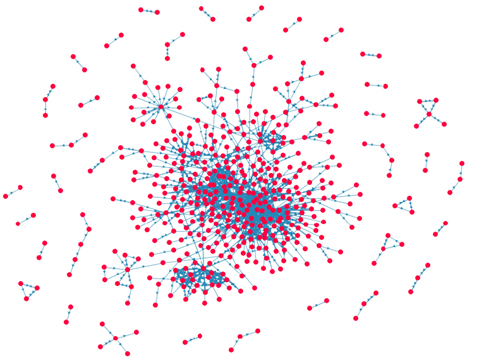
\includegraphics[width=4cm]{images/scattered}}
    }
    \footnote{Picture a, copyright Jennifer Golbeck}%
    \qquad
    \subfloat[Then]{{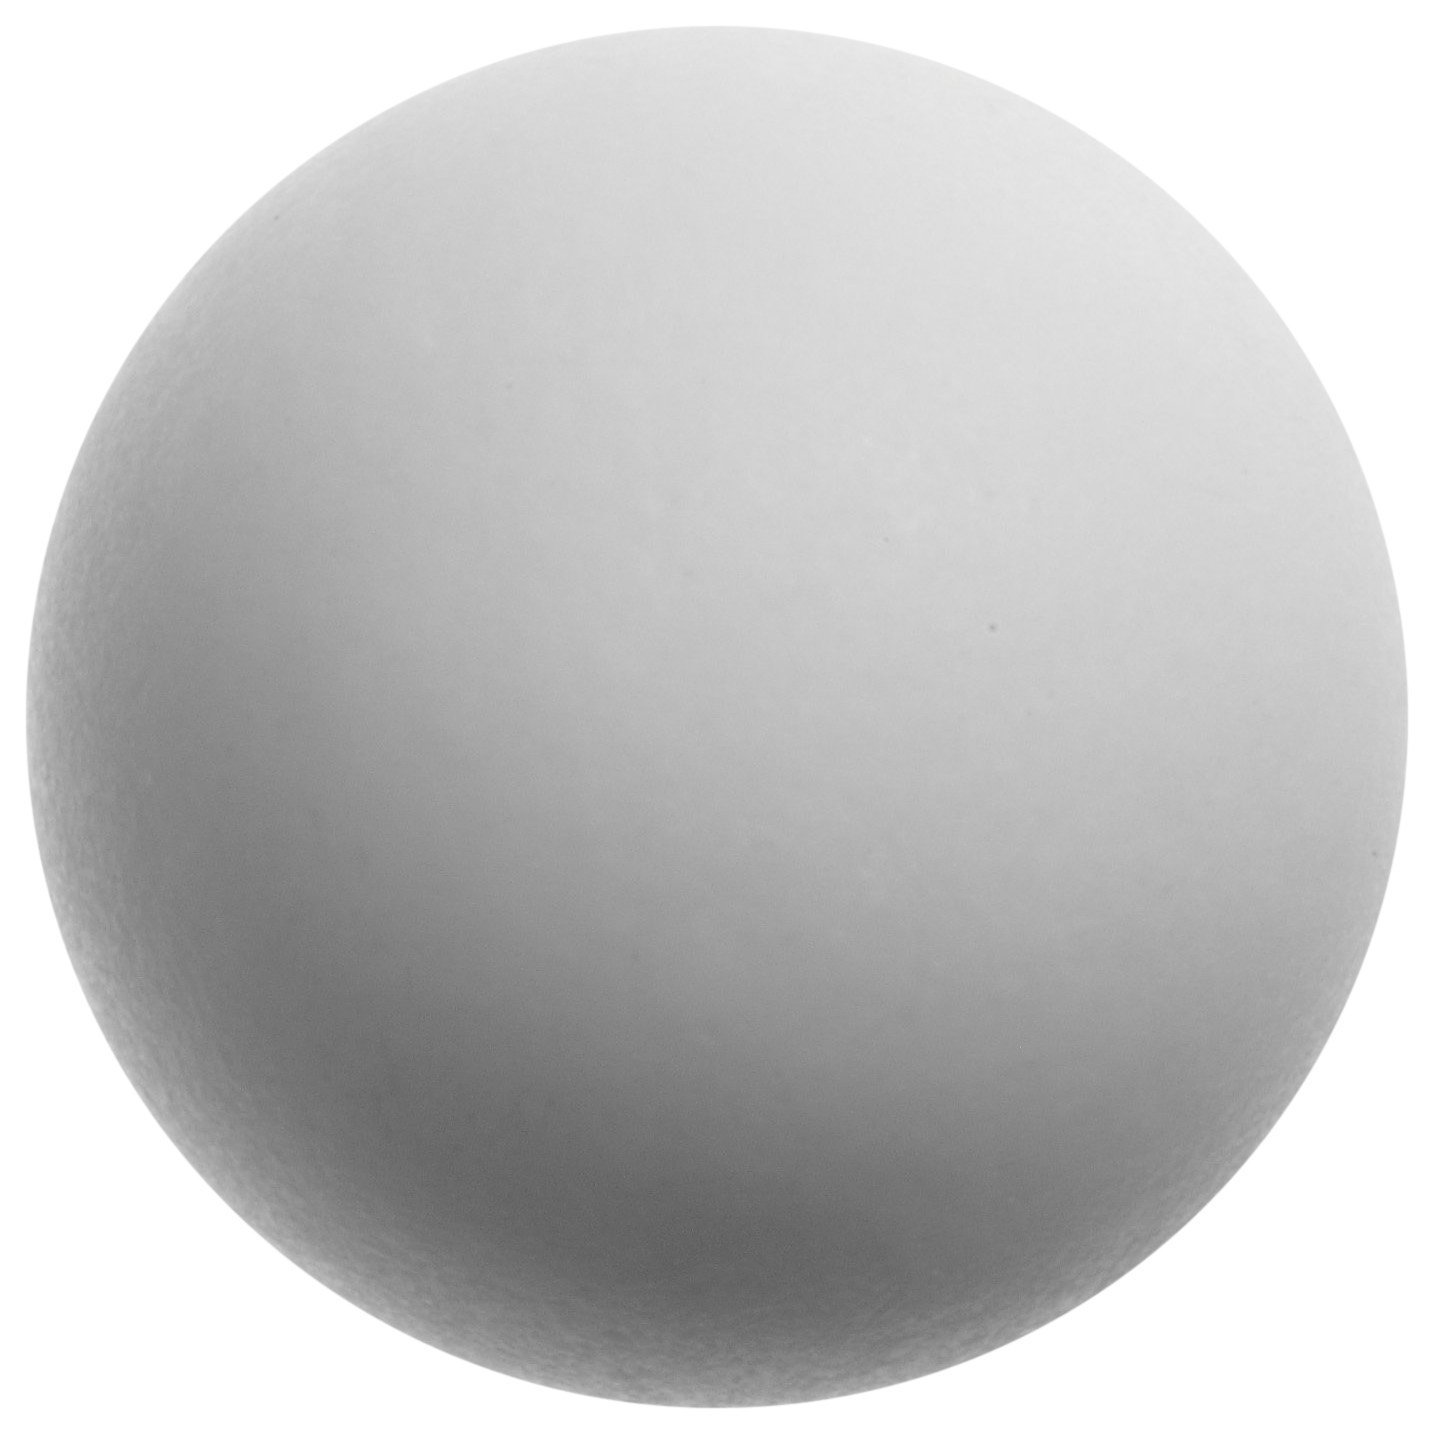
\includegraphics[width=4cm]{images/sphere}}%
    }
    \footnote{picture b, copyright a2ua.com}%
    \label{fig:example}%
\end{figure}
\end{frame}
\end{document}